%iffalse
\let\negmedspace\undefined
\let\negthickspace\undefined
\documentclass[journal,12pt,twocolumn]{IEEEtran}
\usepackage{cite}
\usepackage{amsmath,amssymb,amsfonts,amsthm}
\usepackage{algorithmic}
\usepackage{graphicx}
\usepackage{textcomp}
\usepackage{xcolor}
\usepackage{txfonts}
\usepackage{listings}
\usepackage{enumitem}
\usepackage{mathtools}
\usepackage{gensymb}
\usepackage{comment}
\usepackage[breaklinks=true]{hyperref}
\usepackage{tkz-euclide} 
\usepackage{listings}
\usepackage{gvv}                                        
\def\inputGnumericTable{}                                 
\usepackage[latin1]{inputenc}                                
\usepackage{color}                                            
\usepackage{array}                                             
\usepackage{longtable}                                       
\usepackage{calc}                                             
\usepackage{multirow}                                         
\usepackage{hhline}                                           
\usepackage{ifthen}                                           
\usepackage{lscape}
\usepackage{multicol}

\newtheorem{theorem}{Theorem}[section]
\newtheorem{problem}{Problem}
\newtheorem{proposition}{Proposition}[section]
\newtheorem{lemma}{Lemma}[section]
\newtheorem{corollary}[theorem]{Corollary}
\newtheorem{example}{Example}[section]
\newtheorem{definition}[problem]{Definition}
\newcommand{\BEQA}{\begin{eqnarray}}
\newcommand{\EEQA}{\end{eqnarray}}
\newcommand{\define}{\stackrel{\triangle}{=}}
\theoremstyle{remark}
\newtheorem{rem}{Remark}
\begin{document}

\bibliographystyle{IEEEtran}
\vspace{3cm}

\title{Assignment-2}
\author{EE224BTECH11044 - Muthyala Koushik% <-this % stops a space
}
\maketitle
\newpage
\bigskip

\renewcommand{\thefigure}{\theenumi}
\renewcommand{\thetable}{\theenumi}
\textbf{\section{Vector Arithmetic(CBSE)}}
\begin{enumerate}

    \item If $\brak{3,3},\brak{6,y},\brak{x,7}$ and $\brak{5,6}$ are the vertices of a parallelogram taken in order, find the values of $x$ and $y$. \hfill(10,2011) \\  

\solution To find $x$ and $y$, use the property that the midpoints of the diagonals of parallelogram are equal.
Given vertices:$\vec{A}\myvec{3\\3},\vec{B}\myvec{6\\y},\vec{C}\myvec{x\\7},\vec{D}\myvec{5\\6}$.
$$\text{Midpoint of }\vec{AC}:\myvec{\frac{3+x}{2}\\5}$$
$$\text{Midpoint of }\vec{BD}:\myvec{\frac{11}{2}\\\frac{y+6}{2}}$$
Equate midpoints:
$$\frac{3+x}{2}=\frac{11}{2}\implies x=8$$
$$5=\frac{y+6}{2}\implies y=4$$
So, $x=8$ and $y=4$

\begin{figure}[h!]
	\centering
	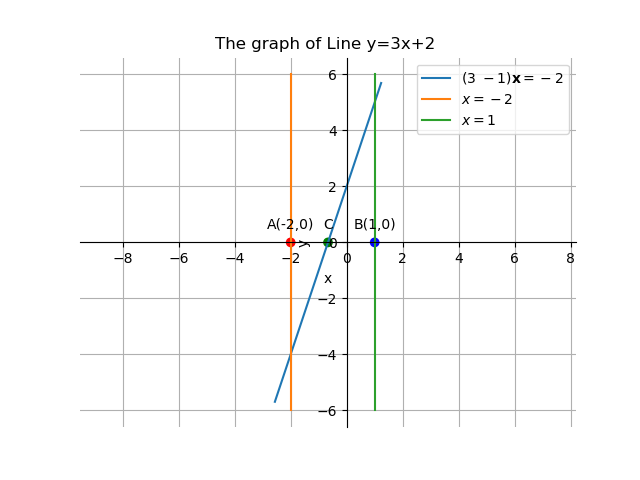
\includegraphics[width=0.7\linewidth]{figs/fig-1.png}
\end{figure}

\end{enumerate}

\end{document}
